% Sandia National Laboratories is a multimission laboratory managed and
% operated by National Technology & Engineering Solutions of Sandia, LLC, a
% wholly owned subsidiary of Honeywell International Inc., for the U.S.
% Department of Energy’s National Nuclear Security Administration under
% contract DE-NA0003525.

% Copyright 2002-2024 National Technology & Engineering Solutions of Sandia,
% LLC (NTESS).


%%
%% MOSFET Table
%%
\small
\begin{longtable}[Hh]{>{\setlength{\hsize}{.4\hsize}}YY} \hline

\underline{\bf General Form} &
\verb|M<name> <drain node> <gate node> <source node>|
\verb|+ <bulk/substrate node> <model name> |

\verb|+ [L=<value>] [W=<value>] |

\verb|+ [AD=<value>] [AS=<value>] |

\verb|+ [PD=<value>] [PS=<value>] |

\verb|+ [NRD=<value>] [NRS=<value>] |

\verb|+ [M=<value] [IC=<value, ...>] |
\\ \hline
\underline{\bf Special Form (BSIMSOI)} &
\verb|M<name> <drain node> <gate node> <source node>|

\verb|+ <substrate node (E)> |

\verb|+ [<External body contact (P)>]|

\verb|+ [<internal body contact (B)>]|

\verb|+ [<temperature node (T)>] |

\verb|+ <model name> |

\verb|+ [L=<value>] [W=<value>] |

\verb|+ [AD=<value>] [AS=<value>] |

\verb|+ [PD=<value>] [PS=<value>] |

\verb|+ [NRD=<value>] [NRS=<value>] [NRB=<value>]|

\verb|+ [BJTOFF=<value>]|

\verb|+ [IC=<val>,<val>,<val>,<val>,<val>] |

\verb|+ [RTH0=<val>] [CTH0=<val>]|

\verb|+ [NBC=<val>] [NSEG=<val>] [PDBCP=<val>] [PSBCP=<val>]|

\verb|+ [AGBCP=<val>] [AEBCP=<val>] [VBSUSR=<val>] [TNODEOUT]|

\verb|+ [FRBODY=<val>] [M=<value>] |

 \\ \hline

\underline{\bf Examples} &
\begin{alltt}
M5 4 12 3 0 PNOM L=20u W=10u
M3 5 13 10 0 PSTRONG
M6 7 13 10 0 PSTRONG M=2
M8 10 12 100 100 NWEAK L=30u W=20u
+ AD=288p AS=288p PD=60u PS=60u NRD=14 NRS=24
\end{alltt} \\ \hline

\underline{\bf Symbols} &
{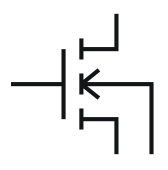
\includegraphics{nmosSymbol}}
{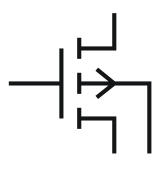
\includegraphics{pmosSymbol}}
\\ \hline

\underline{\bf Model Form} &
\verb|.MODEL <model name> NMOS [model parameters]|
\verb|.MODEL <model name> PMOS [model parameters]|\\ \hline

\underline{\bf Parameters} \underline{\bf and Options} &
\texttt{L} and \texttt{W}
\begin{quote}
  The MOSFET channel length and width that are decreased to get the actual
  channel length and width. They may be given in the device \texttt{.MODEL} or
  \texttt{.OPTIONS} statements. The value in the device statement overrides the
  value in the model statement, which overrides the value in the
  \texttt{.OPTIONS} statement. Defaults for \texttt{L} and \texttt{W} may be
  set in the \texttt{.OPTIONS} statement. If \texttt{L} or \texttt{W} values
  are not given, their default value is 100 u.
\end{quote}
\texttt{AD} and \texttt{AS}
\begin{quote}
  The drain and source diffusion areas. Defaults for \texttt{AD} and
  \texttt{AS} can be set in the \texttt{.OPTIONS} statement.  If \texttt{AD} or
  \texttt{AS} defaults are not set, their default value is 0.
\end{quote}
\texttt{PD} and \texttt{PS}
\begin{quote}
  The drain and source diffusion perimeters. Their default value is 0.
\end{quote}
\\ \hline
\underline{\bf Parameters} \underline{\bf and Options} \bf (cont.) &
% nrg and nrb NOT supported by Xyce, that's a PSPICEism
\texttt{NRD}, \texttt{NRS} 
\begin{quote}
  Multipliers (in units of $\Box$) that can be multiplied by \texttt{RSH}
  to yield the parasitic (ohmic) resistances of the drain (\texttt{RD})
  and source (\texttt{RS}), respectively.  \texttt{NRD}, \texttt{NRS}
  default to 0.

  Consider a square sheet of resistive material. Analysis shows that the
  resistance between two parallel edges of such a sheet depends upon its
  composition and thickness, but is independent of its size as long as it is
  square. In other words, the resistance will be the same whether the square's
  edge is 2~mm, 2~cm, or 2~m. For this reason, the \emph{sheet resistance} of
  such a layer, abbreviated \texttt{RSH}, has units of ohms per square,
  written $\mathsf{\Omega}/\Box$.
\end{quote}
\texttt{M}
\begin{quote}
  If specified, the value is used as a number of parallel MOSFETs to
  be simulated.  For example, if \texttt{M}=2 is specified, we
  simulate two identical mosfets connected to the same nodes in
  parallel.
\end{quote}
\texttt{IC}
\begin{quote}
  The BSIM3 (model level 9), BSIM4 (model level 14) and BSIMSOI (model level 
  10) allow one to specify the initial voltage difference across nodes of the 
  device during the DC operating point calculation.  For the BSIM3 and BSIM4
  the syntax is \texttt{IC= $V_{ds}, V_{gs}, V_{bs}$} where $V_{ds}$ is the 
  voltage difference between the drain and source, $V_{gs}$ is the voltage 
  difference between the gate and source and $V_{bs}$ is the voltage difference 
  between the body and source.   The BSIMSOI device's initial condition syntax 
  is \texttt{IC= $V_{ds}, V_{gs}, V_{bs}, V_{es}, V_{ps}$} where the two extra 
  terms are the voltage difference between the substrate and source, and the 
  external body and source nodes respectively.  Note that for any of these 
  lists of voltage differences, fewer than the full number of options may be 
  specified.
\end{quote}

\\ 
& 
\begin{quote} 
  For example, \texttt{IC=5.0} specifies an initial 
  condition on $V_{ds}$ but does not specifiy any initial conditions on the other
  nodes.  Therefore, one cannot specify $V_{gs}$ without specifying $V_{ds}$, etc.  
  It is illegal to specify initial conditions on any nodes that are tied together.
  \Xyce{} attempts to catch such errors, but complex circuits may stymie this
  error trap. 
\end{quote} 

\\ \hline

\underline{\bf BSIMSOI-specific} \underline{\bf Options} &

There are a large number of extra instance parameters and optional
nodes available for the BSIMSOI (level 10) MOSFET.

\texttt{substrate node}
\begin{quote}
The fourth node of the BSIMSOI device is always the substrate node, which 
is referred to as the \texttt{E} node.
\end{quote}

\texttt{external body contact node}
\begin{quote}
If given, the fifth node is the external body contact node, {\texttt
P}.  It is connected to the internal body node through a body tie
resistor.  If \texttt{P} is not given, the internal body node is not
accessible from the netlist and floats.

If there are only five nodes specified and \texttt{TNODEOUT} is also specified, the fifth node is the temperature node instead.
\end{quote}

\texttt{internal body contact node}
\begin{quote}
If given, the sixth node is the internal body contact node, {\texttt
B}.  It is connected to the external body node through a body tie
resistor.  If \texttt{B} is not given and \texttt{P} is given, the internal 
body node is not accessible from the netlist, but is still tied to the 
external body contact through the tie resistance.

If there are only six nodes specified and \texttt{TNODEOUT} is also specified, the sixth node is the temperature node instead.
\end{quote}

\texttt{temperature node}
\begin{quote}
If the parameter \texttt{TNODEOUT} is specified, the final node (fifth, sixth, or seventh) is interpreted as a temperature node.  The temperature node is intended for thermal coupling simulation.
\end{quote}

\texttt{BJTOFF}
\begin{quote}
Turns off the parasitic BJT currents.
\end{quote}

\texttt{IC}
\begin{quote}
The \texttt{IC} parameter allows specification of the five junction initial conditions, VDS, VGS, CBS, VES and VPS.  VPS is ignored in a four-terminal device.
\end{quote}

\\ \hline 
\underline{\bf BSIMSOI-specific} \underline{\bf Options} {\bf (cont.)} &

\texttt{RTH0}
\begin{quote}
Thermal resistance per unit width.  Taken from model card if not given.
\end{quote}

\texttt{CTH0}
\begin{quote}
Thermal capacitance per unit width.  Taken from model card if not given.
\end{quote}

\texttt{NBC}
\begin{quote}
Number of body contact isolation edge.
\end{quote}

\texttt{NSEG}
\begin{quote}
Number of segments for channel width partitioning.
\end{quote}

\texttt{PDBCP}
\begin{quote}
Parasitic perimeter length for body contact at drain side.
\end{quote}

\texttt{PSBCP}
\begin{quote}
Parasitic perimeter length for body contact at source side.
\end{quote}

\texttt{AGBCP}
\begin{quote}
Parasitic gate-to-body overlap area for body contact.
\end{quote}

\texttt{AEBCP}
\begin{quote}
Parasitic body-to-substrate overlap area for body contact.
\end{quote}

\texttt{VBSUSR}
\begin{quote}
Optional initial value of VBS specified by user for use in transient analysis.
(unused in \Xyce{}).
\end{quote}

\texttt{FRBODY}
\begin{quote}
Layout-dependent body resistance coefficient.
\end{quote}

\\ \hline

\underline{\bf Comments} & The simulator provides three MOSFET device models,
which differ in the formulation of the I-V characteristic. The \texttt{LEVEL}
parameter selects among different models as shown below.
\\ \hline
\end{longtable}

% Eric Keiter.  1/19/04:
% As this table does not have a caption, it should not have a number
% assigned to it.  This line is needed to fix latex so that the tables in
% chapter 2, which actually have their numbers printed in table captions, 
% and the list of tables,  do not start at 2.9, but start at 2.1.
\addtocounter{table}{-1}


